\documentclass[a4paper, 12pt]{report}

% Adapté du tempate TER-M1 de l'Université de Paris

%%%%%%%%%%%%
% Packages %
%%%%%%%%%%%%

\usepackage[french]{babel}
%\usepackage{hyperref}
\usepackage[noheader]{packages/sleek}
\usepackage{packages/sleek-title}
\usepackage[french]{packages/sleek-theorems}
\usepackage{packages/sleek-listings}
\usepackage{tikz}
\usepackage[french,lined]{algorithm2e}	
\usepackage{pdfpages}
\usepackage{graphicx}
\graphicspath{ {./images/} }

\SetKwInput{KwResult}{R\'esultat}
\SetKw{KwInput}{Entr\'ees}
%%%%%%%%%%%%%%
% Title-page %
%%%%%%%%%%%%%%

\logo{./resources/img/logo_science.png}
\institute{Sorbonne Université}
\faculty{Master ANDROIDE}
\title{Apprentissage social et imitation pour la robotique en essaim}
\subtitle{UE de projet M1}
\author{Alessia \textsc{Loi} -- Dorian \textsc{LANCELIN}}
\date{2022}



%%%%%%%%%%%%%%%%https://www.overleaf.com/project/6012bd305aee4065605e8f1d
% Bibliography %
%%%%%%%%%%%%%%%%

\addbibresource{./resources/bib/references.bib}

%%%%%%%%%%
% Others %
%%%%%%%%%%

\lstdefinestyle{latex}{
    language=TeX,
    style=default,
    %%%%%
    commentstyle=\ForestGreen,
    keywordstyle=\TrueBlue,
    stringstyle=\VeronicaPurple,
    emphstyle=\TrueBlue,
    %%%%%
    emph={LaTeX, usepackage, textit, textbf, textsc}
}

\FrameTBStyle{latex}

\def\tbs{\textbackslash}

%%%%%%%%%%%%
% Document %
%%%%%%%%%%%%

\begin{document}
    \maketitle
    \romantableofcontents

    \chapter{Introduction}

    -On cherche à trouver des outils permettant à des robots avec une mémoire très limitée d'apprendre à réaliser une tâche par observation des mouvements d'autres robots au mêmes spécifications.
    
    - On considèrera que les robots ont des moyens de communication limités voire inexistant si possible.
    
    - En utilisant des agents au comportement prédéfini, les experts, capables de réaliser au mieux la tâche envisagée, on arrive toujours à observer une convergeance vers le comportement de l'expert dans les cas où l'apprentissage se fait uniquement dans le sens expert-apprenant.
    Dans certains cas particuliers, des méthodes explorées permettent a l'apprentissage apprenant-apprenant d'accélerer cette convergeance. 
    
    Ce projet a été encadré par messieurs Nicolas Bredeche et Stéphane Doncieux.  
    
    L'ensemble des codes utilisé afin d'obtenir les résultats décrit dans le document suivant sont disponible sur notre dépôt \href{https://github.com/aerrynn/M1_Projet_ASIRE}{github}. 

    \chapter{État de l'art}
    Un chapitre dédié à l'état de l'art doit décrire les concepts et méthodes déjà existant(e)s, en lien avec le travail que vous avez réalisé.
    
    \chapter{Contribution}
   
    \section{Choix de l'expérimentation : La tâche de fourragement}
    Dans le but d'évaluer la capacité d'apprentissage par comportement de notre essaim de robots, on a reproduit l'expérience de fourragement et simulée à l'aide de pyRoborobo.
    L'évaluation en elle-même se fait sur la quantité d'objets capturés par un agent sur une fenêtre de temps donnée (sliding window). On considèrera qu'il n'y a pas de perte d'information lors du transfert, c'est à dire que l'apprenant est capable de voir tout ce que voit l'expert.
    On définit ainsi les paramètres de l'expérience :
    \begin{itemize}
    \item Taille de la population : 100
    \item Nombre d'experts : 10
    \item Nombre d'apprenants : 90
    \item Nombre d'objets : 100
    \item Taille de l'arène : 1400x800
    \item Taille des robots : 5x5
    \item Nombre de senseurs : 16
    \item Distance des senseurs : 16
    \item Durée d'une expérience : 20,000
    \item Nombre de répétion de l'expérience : 5
    \end{itemize}
    
// Mentionner qu'on utilise les senseurs étendus (dim. 24) donnant de l'info sur dist robots, dist objets, dist murs.

Les différents experts suivent un comportement donné.
// Algo comportement 1 : sous forme de génome

// Algo comportement 2
L'objectif de ce comportement est d'éviter les obstacles (qu'ils soient des murs ou d'autres robots) tout en se focalisant sur le ramassage des objets dès que possible.

	\section{Méthodes explorées}
	Les méthodes que nous avons étudié pour implementer la diffusion de compétences au sein de la population sont les suivantes :
	\begin{itemize}
	\item Méthode par transmission de comportements.  
	La transmission de comportements est une approche algorithmique deterministe qui fait correspondre à chaque état de l'environnement (input) une et une seule action à effectuer exprimée sous forme de contrôles moteur (output) determinant le mouvement du robot.
	
	\item Méthode par mimétisme
	\end{itemize}
	
	\section{Méthode par transmission de comportements}
	On considère que chaque individu robot possède une base de données de traces comportamentales, utile à stocker les comportements que un individu expert lui a envoyé lorsque les deux robots ont croisé leurs trajectoires.
	
	La base de données de chaque individu expert est initialisée au début de l'experience : elle contient 100 traces définies et n'evolue pas au cours du temps. Parmi toutes les traces possibles, les 100 traces que nous avons sélectionné permettent aux individus experts d'être efficaces dans l'évitement de murs, l'évitement des robots pour prevenir les interblocages et la collecte d'objets lorsqu'un objet se trouve dans le perimètre perceptible par les senseurs.
	
	Une trace comportementale est un doublet $( s_t, a_t )^T$, avec :
	\begin{itemize}
	\item $s_t$ : l'état courant du contexte, qui correspond à une liste de 24 valeurs des senseurs étendus. L'état courant est de la forme 
    $(s_1, s_2, s_3, ..., s_n)$ avec $n$ le nombre de senseurs du robot. 
	\item $a_t$ : l'action à appliquer en fonction du contexte sensoriel rélévé. L'action associée est de la forme $[t,r]$ avec $t$ le degré de transition et $r$ le dégré de rotation.
	\item $T$ : le temps de croisement des deux trajectoires, exprimé en nombre de steps. 
	\end{itemize}


	La base de données de chaque individu focal évolue au cours du temps. Au depart elle contient une seule trace correspondant à un comportement par défaut à appliquer lorsque aucun des senseurs ne perçoit aucun élement de l'énvironnement. Chaque fois que les trajectoires d'un individu focal et d'un individu expert se croisent, l'expert envoie une partie de ses traces à l'individu focal, qui enrichit ainsi sa collection de traces.
	
    L'ensemble de traces comportamentales d'un individu focal constitue la base d'exemples (senseurs) et étiquettes (actions) qui sera utilisée pour l'entrainement et la prediction des algorithmes d'apprentissage.
    
    \:
    
    \textbf{Protocole experimental specifique à cette partie.} A chaque debut d'evaluation, les conditions initiales sont réinitialisées, notamment:
    \begin{itemize}
	\item la position de tous les individus;
    \item la base de données de comportements;
    \item la performance de chaque individu, exprimée en nombre d'objets collectés.
	\end{itemize}
    
    Remarque : pour l'algorithme de rétropropagation du gradient, les poids du réseau de neurones ne seront pas réinitialisées entre une évaluation et l'autre, dans le but de raffiner les poids precedemment obtenus en les testant sur un nouveau contexte.
    
    Les graphiques de distance sont obtenus ainsi:
    \begin{itemize}
        \item Nous capturons l'univers aperçu par un individu expert, en enregistrant l'état qu'il détecte (liste de 24 senseurs) et la correspondante action effectuée à chaque step.
        \item A $t = 1000$ steps, nous utilisons la connaissance actuelle du meilleur individu focal (poids du réseau de neurones ou état courant de la base de données de traces comportamentales) pour collecter la prediction (liste d'actions) sur les états de l'expert. La distance est la distance euclidienne entre l'action de l'expert et l'action du meilleur individu focal.
        \item Nous répetons la même technique à $t = 2500$ steps et à $t = 6000$ steps, ensuite nous comparons les résutats sur la tranche de $t = 0$ steps à $t = 2500$ steps.
    \end{itemize}


	
	
    \subsection{Apprentissage par rétropropagation du gradient}
    L'apprentissage par rétropropagation du gradient permet d'observer une évolution fluide du comportement des individus focaux : les trajectoires dessinent des ellipses qui deviennent progressivement plus larges et ouvertes au cours du temps. En presence d'obstacles, les individus répondent rapidement pour l'évitement des murs et nous observons qu'il ne se vérifie pas d'interblocage avec les autres robots. De manière moins importante par rapport aux experts, nous remarquons aussi la réconnaissance d'objets.
    
    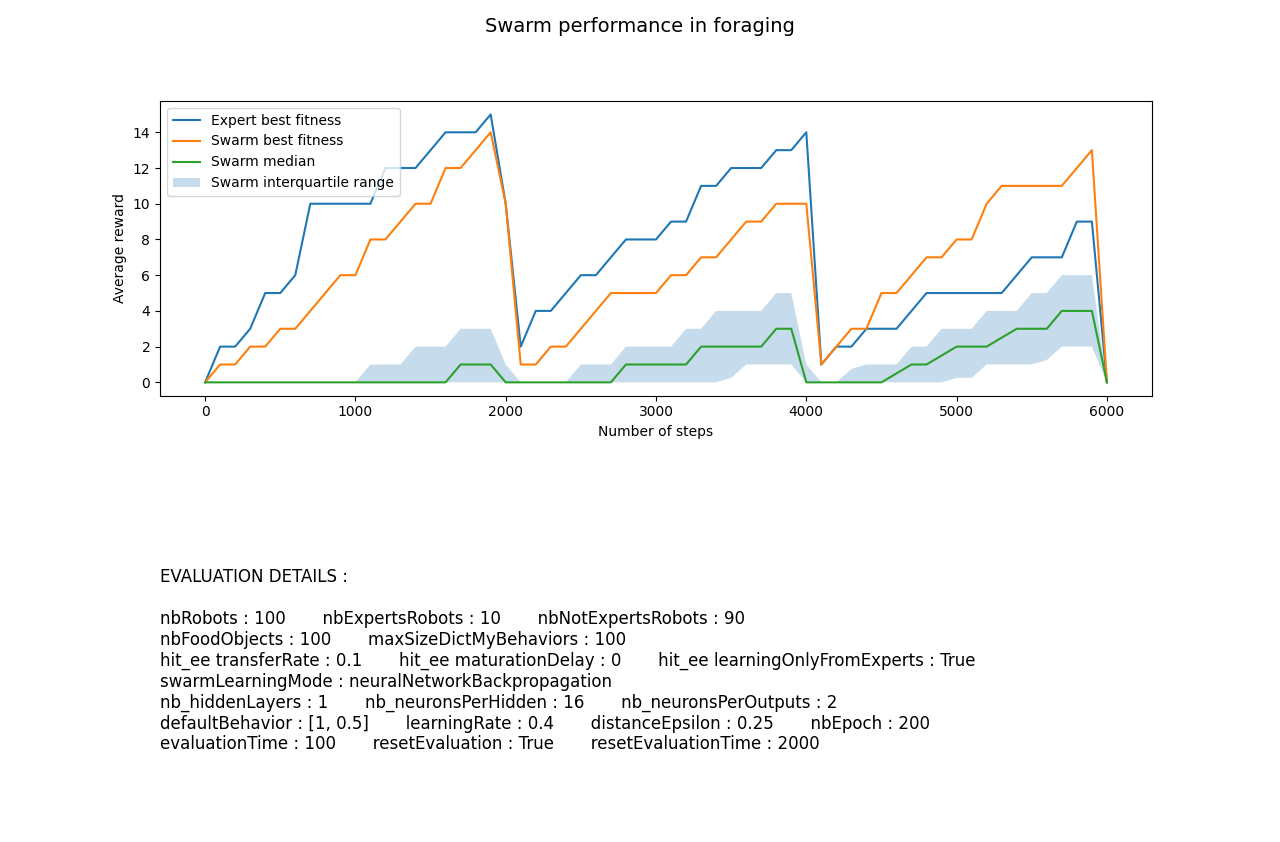
\includegraphics[scale=0.5]{bp6000_100.png}
    
    L'apprentissage par rétropropagation du gradient se révèle efficace et confère à chaque individu un mouvement continu qui n'imite pas parfaitement le comportement de l'expert mais assure la poursuite des mêmes objectifs. Cette proprièté permet parfois d'avoir des résultats meilleurs en termes de performance par rapport à ceux des experts. 
    Dans le graphique on observe que à la troisième évaluation le meilleur individu non expert de l'essaim obtient une meilleure performance par rapport à celle de l'expert observé. On remarque aussi la progressive amélioration de la performance des individus non experts.


    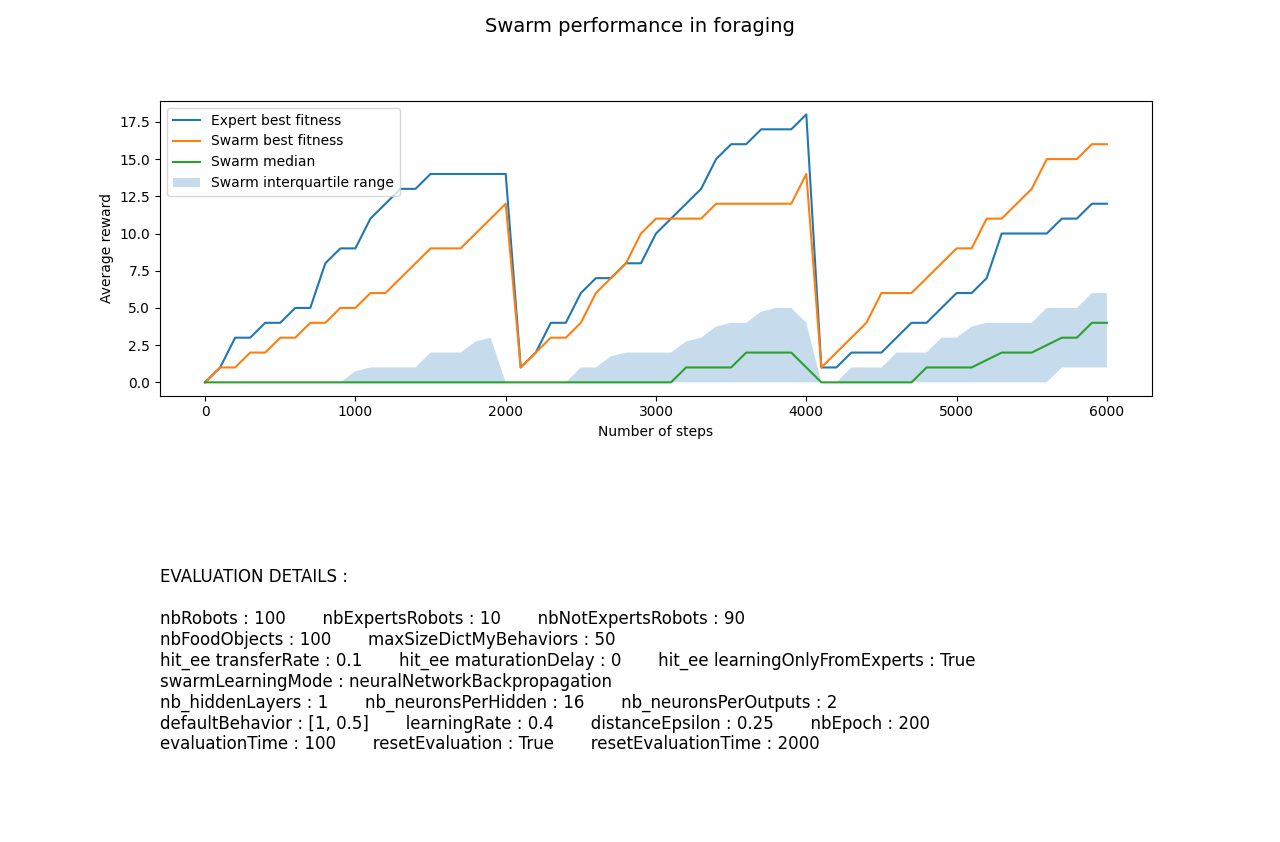
\includegraphics[scale=0.5]{bp6000_50.png}

    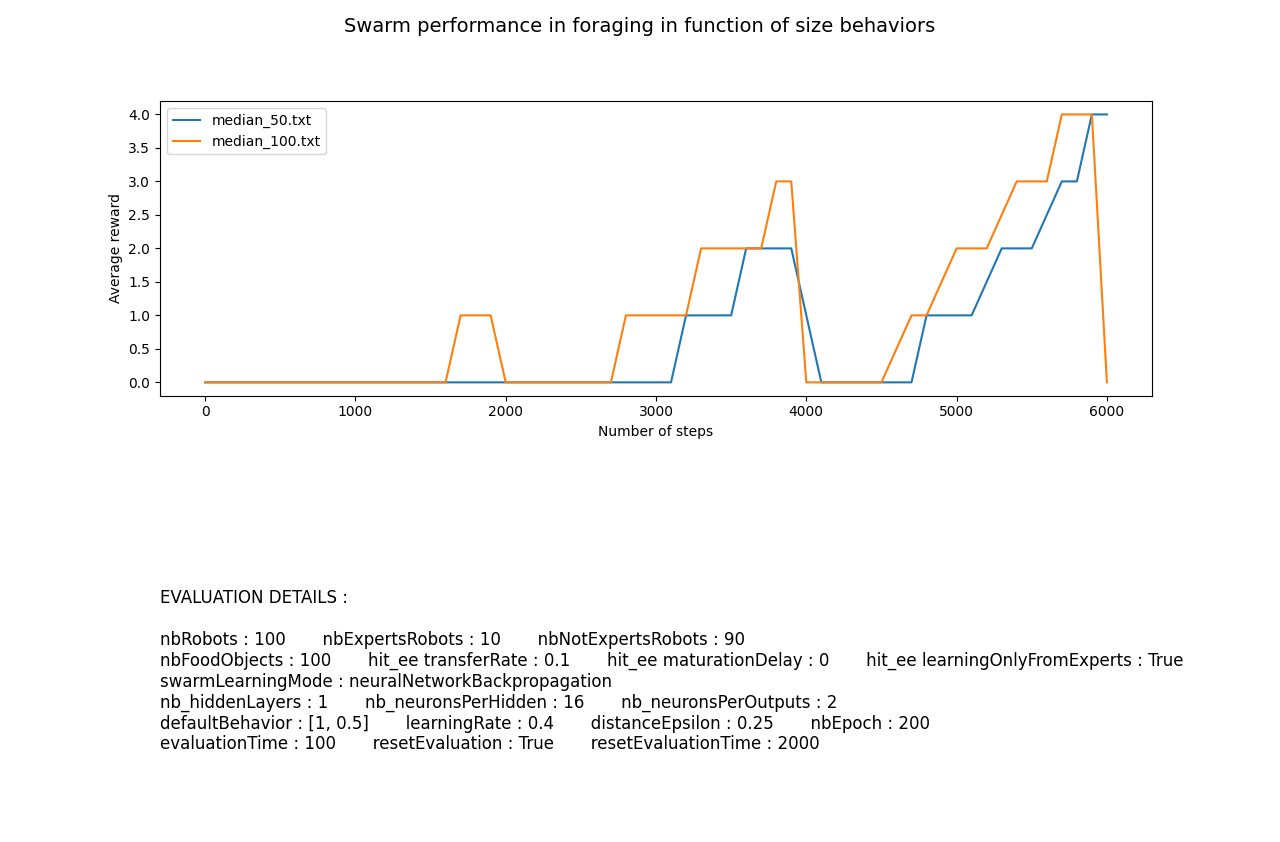
\includegraphics[scale=0.5]{sizeDB_50vs100_bp.png}

    La limitation de la base de données des individus focaux à 50 éléments (sur 100 traces totales possiblement acquérable depuis les experts) réduit légèrement la capacité de l'essaim d'apprendre de l'expert. 


    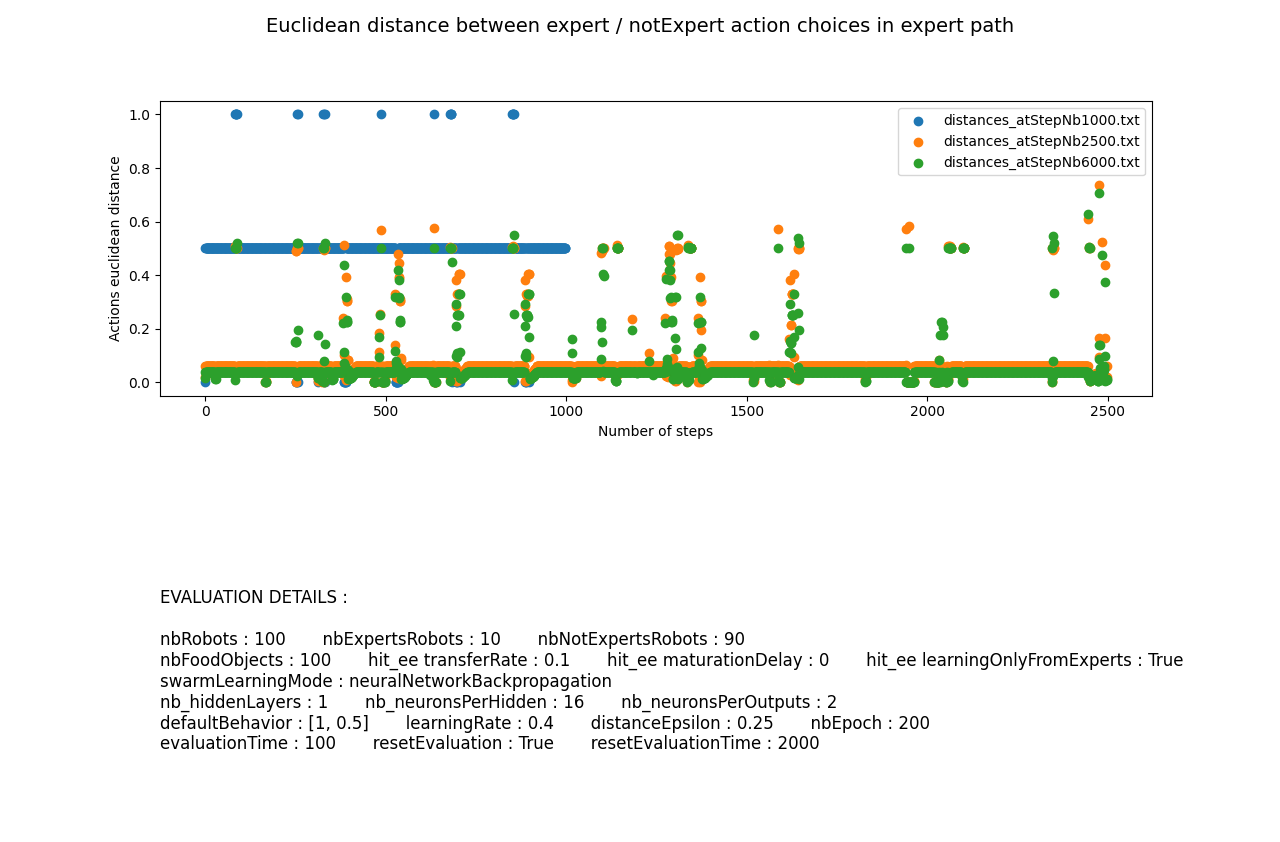
\includegraphics[scale=0.5]{distances_bp.png}

    Les choix effectuées par le meilleur individu focal en termes d'actions s'améliorent au cours du temps. La bande verte répresente une distance minimale entre l'action de l'indivudu focal et l'action de l'expert au moment $t = 6000$ step.
    Nous remarquons que le meilleur individu focal avait déjà trouvé des poids efficaces pour le réseau de neurones au moment $t = 2500$ step. 





    \subsection{Apprentissage par k Plus Proches Voisins}
    L'apprentissage par k Plus Proches Voisins permet d'observer une modification nette des comportements chez les individus focaux : les trajectoires changent rapidement suite à la phase d'entrainement, et ressemblent au comportement d'un individu expert. Cela est dû au fait que chaque action sélectionnée par l'apprentissage de l'individu focal correspond exactement à au moins une action de la base de données de l'expert, sans perte d'information.
    
    
    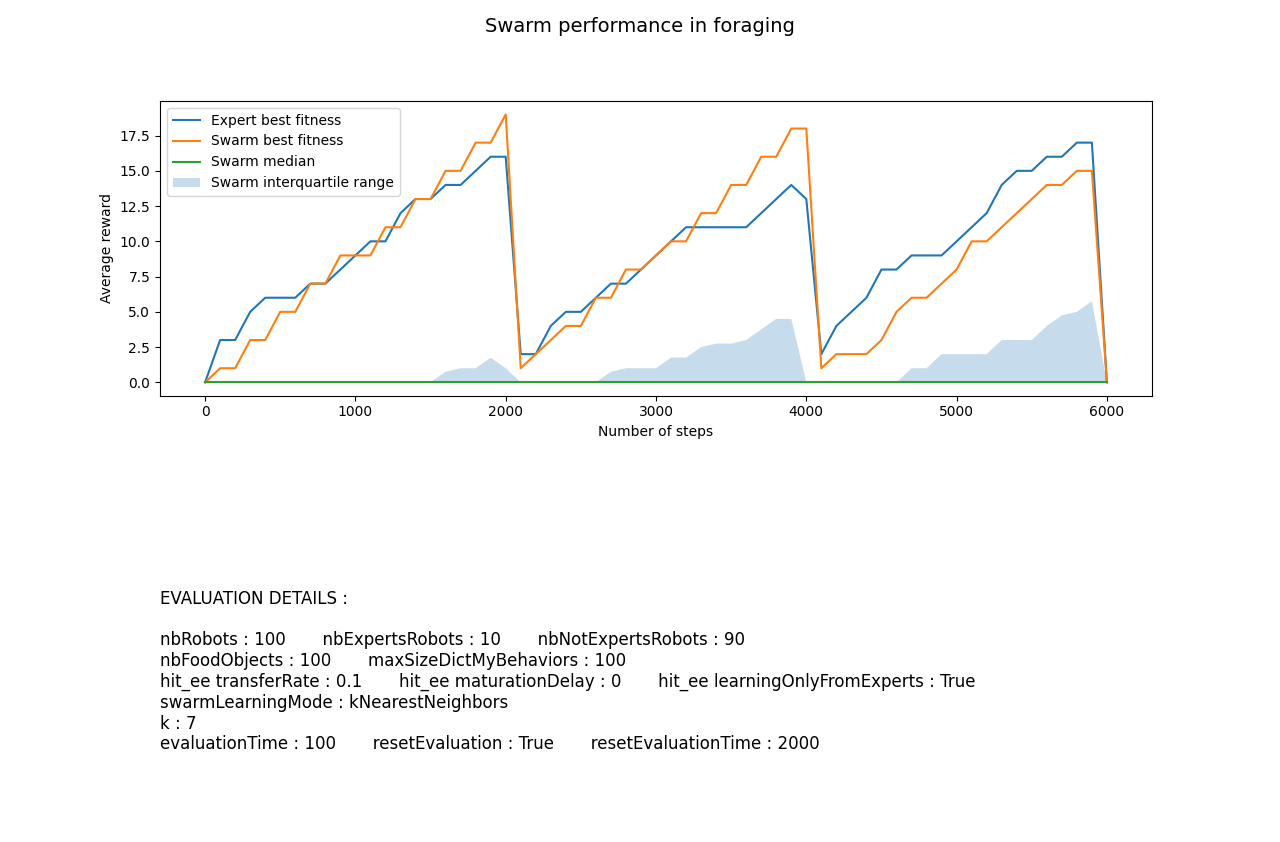
\includegraphics[scale=0.5]{knn6000_100.png}
    
    L'apprentissage par k Plus Proches Voisins est efficace et tend à imiter parfaitement le comportement de l'expert.
    Dans le graphique, nous pouvons voir que la performance du meilleur individu focal et de l'expert sont presque superposées. La connaissance génerale du groupe évolue en fonction du temps mais progresse moins vite par rapport à l'apprentissage par rétropropagation du gradient.
    
    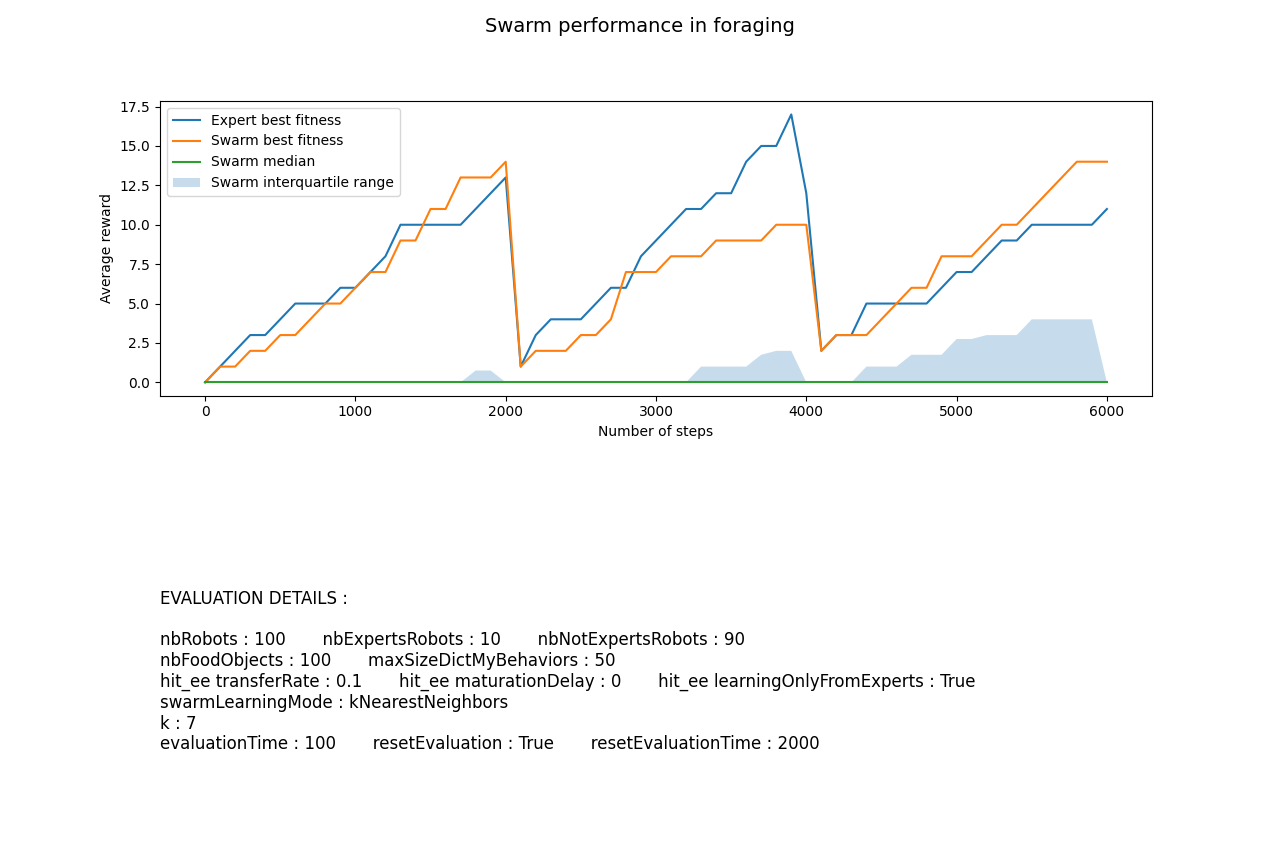
\includegraphics[scale=0.5]{knn6000_50.png}
    
    La limitation de la base de donnée des individus focaux à 50 éléments (sur 100 traces totales possiblement acquérable depuis les experts) réduit la capacité de l'essaim d'apprendre de l'expert. 
    
    
    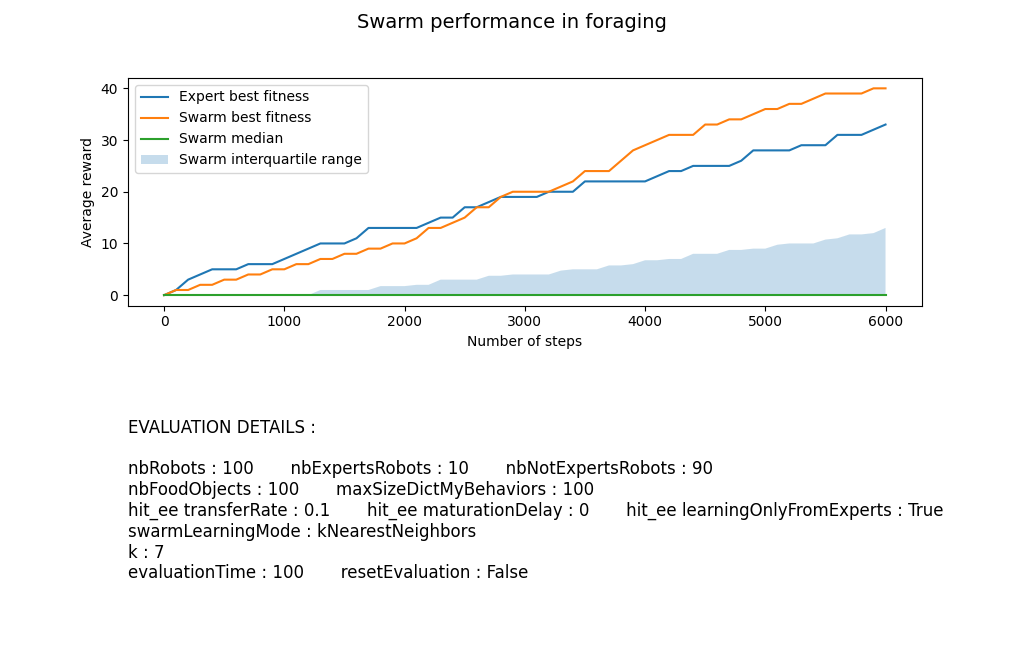
\includegraphics[scale=0.5]{knn6000_100_noReset.png}
        
    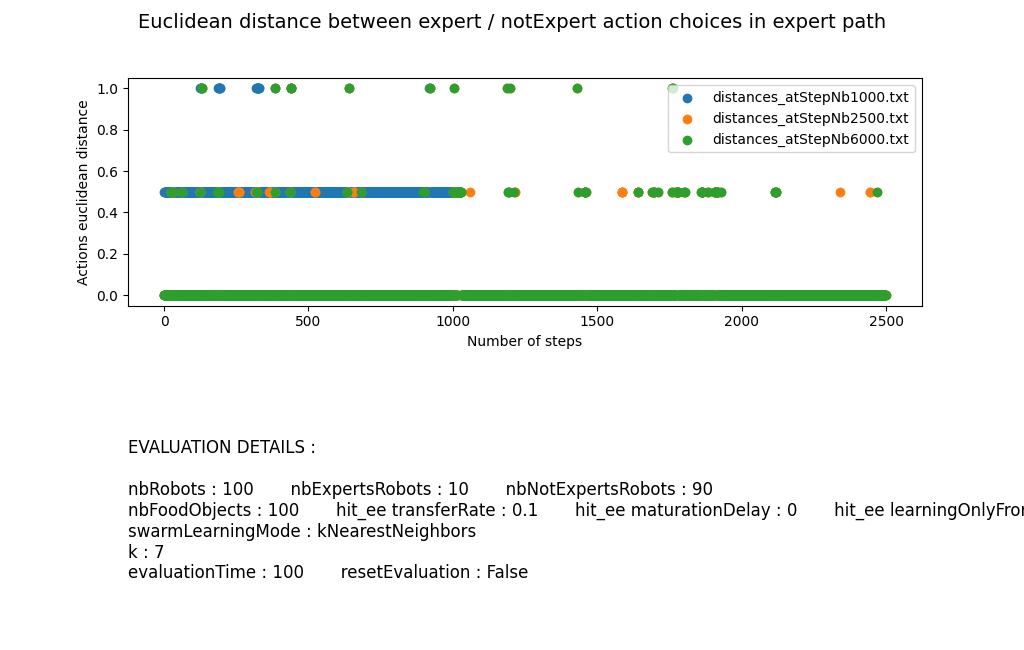
\includegraphics[scale=0.5]{distances_knn.png}
    
    Ce graphique des distances entre actions est obtenu à partir de l'expèrimentation de 6000 steps sans réinitialisation des conditions initiales representée juste en dessus. Nous remarquons qu'en fin d'évaluation l'essaim a un comportement beaucoup plus proche à celui de l'expert - en termes de actions choisies - par rapport au debut d'évaluation.
    
    
    
    
    
	\section{Méthode par mimétisme}
	On décide ensuite de généraliser l'apprentissage en ajoutant de nouvelle contraintes : pour qu'un individu apprenne un comportement, ce dernier doit être observé. On change ainsi les informations transmises lors de la rencontre entre deux individus en un couple (observation, action) envoyé par l'expert.
	Pour simplifier on ne considère pas la perte d'information due au changement de point de vue.
	\subsection{Apprentissage ad-hoc}
	Dans un premier temps, on se propose d'évaluer l'apprentissage par mimétisme en donnant aux apprenants une mémoire extensible et en déterminant le comportement des agents non-experts de la manière suivante :

\fbox{
	\begin{algorithm}[H]
		\KwInput{une observation $o$}\;
		\KwResult{l'action à effectuer $a$ }
  		On cherche l'observation $o'$ présente dans la mémoire telle que la distance $o$-$o'$ soit minimale\;
		L'observation $o'$ étant stockée avec une action $a'$ associée : $a$ $\leftarrow$ $a'$ \;
  		return $a$\;
	\end{algorithm}}
	
	La première remarque que l'on peut faire sur cette méthode d'apprentissage est qu'au délà d'être coûteuse en mémoire, la simulation dure très longtemps du fait que les observations appartiennent à des segments continus compris entre 0 et 1.
	
	De plus, lorsqu'un apprenant apprend un comportement, celui-ci est toujours dans le rayon de perception de l'expert, ce qui entraine une perte de généralisation. Par exemple les situation où un agent se retrouve en face d'un objet sans qu'aucun autre agent ne soit détecté par ses senseurs ne peuvent être apprises.
	Pour palier à ce problème, dans un premier temps, on a fait le choix de ne transmettre que les informations des capteurs frontaux.
	Lorsque l'on ajoute l'apprentissage inter-apprenants, on observe rapidement à un problème : un agent non-expert peut apprendre un mauvais comportement et l'on a -pour l'instant - aucun moyen de filtrer ou d'éliminer ces comportements sub-optimaux.
	
	\subsection{apprentissage ad-hoc avec discrétisation des entrées}
	Afin d'adapter la méthode ad-hoc au domaine de la robotique en essaim, et donc de limiter la mémoire nécessaire, on a essayé de discrétiser les entrer. Une telle méthode a plusieur avantage : elle réduit le domaine des observations $$nombre d'intervalles^{nombre de senseurs}*2^{nombre de senseurs de typage} $$ et permet de hasher ces dernière pour accéder plus efficacement aux comportements.
	Pour cette version, le comportement des apprenants suit les règles suivante :
	
\fbox{
\begin{algorithm}[H]
	\KwInput{une observation $o$}\;
	\KwResult{l'action à effectuer $a$ }
	$o'$ $\leftarrow$ Discrétiser($o$)\;
	\If{o' est une clé du dictionnaire $mémoire$}								
	{\Return mémoire[$o'$]}
	\Return mouvement par défaut\;
\end{algorithm}}
	
	
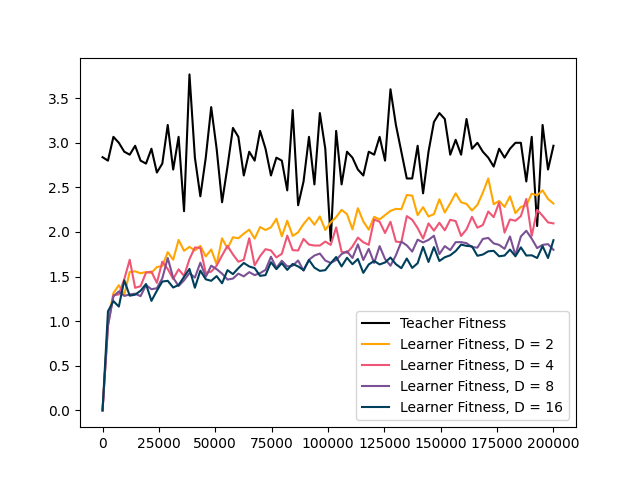
\includegraphics{averageComparisons}


	Par ces analyse, on remaque que lorsque le nombre d'intervalles de discrétisation augmente, la convergeance est de plus en plus lente ce qui s'explique par le plus grand nombre de comportements à apprendre.
	 Cette supposition est confirmé par la quantité de mouvements appris en fonction du nombre d'intervalles de discrétisations.
	 
	 
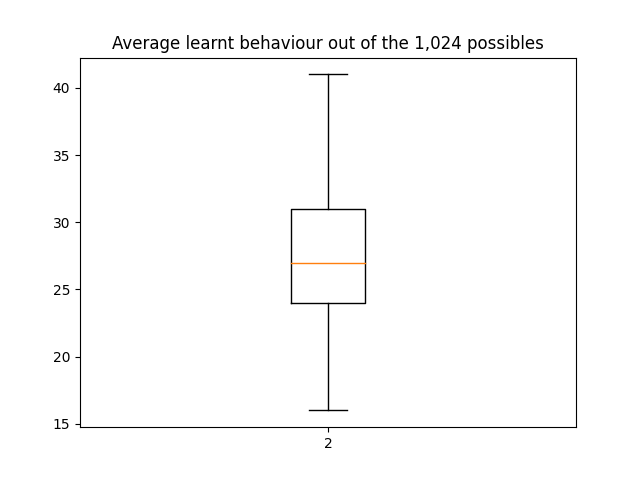
\includegraphics[scale = 0.5]{averageLearntBehaviourD2}
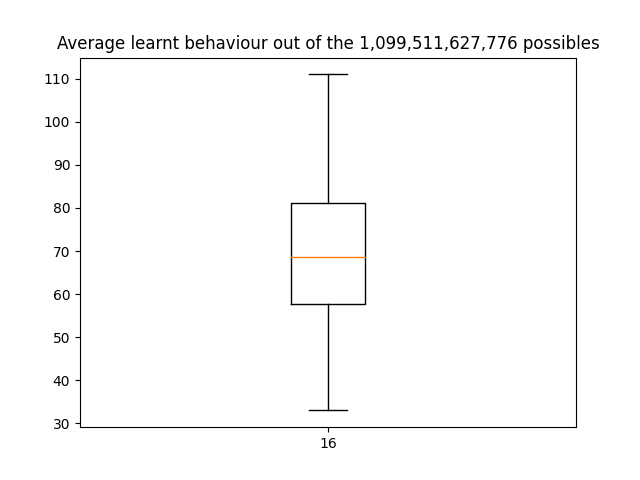
\includegraphics[scale = 0.5]{averageLearntBehaviourD16}
	
	En revanche si le nombre d'intervalles est insuffisant, une partie du comportement de l'expert peut être perdue. Par exemple si un expert adopte trois comportements différents en fonction de la valeur du senseur 1, une discrétisatione en deux intervalles (respectivement [0,0.5], ]0.5,1]) ne permettrait pas l'apprentissage exact de ce comportement.
	
	Pour implémenter la propagation, il suffit de modifier la règle d'apprentissage de la manière suivante :
	
	%// Pseudocode
\fbox{
\begin{algorithm}[H]
	Lors de la réception d'un message $m$\;
	$o$,$a$ $\leftarrow$ $m$
	\If {$a\neq$ action par défaut}{$o'\leftarrow$discrétiser($o$)
	\If {$o'$ n'est pas une clé de du dictionnaire $mémoire$}{$mémoire$[$o'$] $\leftarrow a$}}
\end{algorithm}}
	
	
	\textbf{N.B.}Pour les tests, on a fait le choix de définir le mouvement par défaut comme (0.5, 0.05), c'est à dire de continuer tout droit, mais avec un léger déplacement vers la droite pour éviter de se coincer.

\begin{center}
	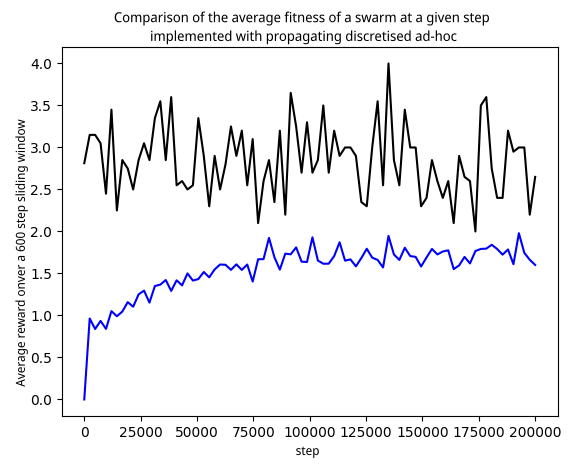
\includegraphics{D2Propag}
\end{center}	
A première vue, cette experience semble donner des résultats moins bons que sans propagation, mais elle n'est pas représentative, car nous avons dû limiter le nombre de répétitions de l'expérience par manque de temps. Il faudrait donc refaire cette expérience en la comparant à sa version sans propagation, et ce sur un nombre représentatif d'expériences.
	
	
	\subsection{Apprentissage ad-hoc avec PPV}
	Une autre option envisagée pour réduire la demande en mémoire de notre algorithme est de toujours exécuter l'action de la mémoire dont l'observation est la plus proche de l'observation actuelle.
	De plus afin de limiter le nombre de points insérés dans la mémoire, on a implémenté l'algorithme suivant :

\fbox{
\begin{algorithm}[H]
	\SetAlgoLined
	Lors de la réception d'un message $m$\;
	$o$,$a$, $w$ $\leftarrow$ $m$
	On cherche le couple ($o'$, $a'$) tel que la distance $o-o'$ soit minimale\;
	\If{$a\neq a'$}{On ajoute le tuple ($o$, $a$, 1) à la mémoire}{On modifie $o$ de la manière suivante\;
	$o'\leftarrow$ ( $ \frac{o'* w + o}{w+1}$}
\end{algorithm}}
	
Les principales différences observées lors de ces tests étaient dues au choix de l'heuristique de calcul de distance. En effet une heuristique de simple calcul de distance euclidienne avait comme défaut de ne pas prendre en compte le type des objets rencontrés (ceux ci étant encodés sous forme de booléens 0,1). Une solution a été d'utiliser une heuristique maximin, mais les resultats restaient insuffisants.
Au final, nous avons fait le choix de projeter les distances aux obstacles sur différents hyperespaces correspondants aux différentes permutations du type d'objet rencontré, puis fait le calcul sur la distance euclidienne.

L'inconvénient majeur de cette méthode est la difficulté à l'adapter à la propagation entre apprenants. Simplement permettre cette dernière provoquerait l'apprentissage de "mauvais" comportements qui limiteraient à long terme la convergence de l'efficacité de la population.

Une solution envisagée à été de calculer pour chaque observation faite la vraisemblance du mouvement associé à cette observation. Mais cette méthode, très calculatoire, demandait une grande mémoire pour avoir une base de comparaison.
	
	\subsection{Apprentissage sur un réseau de Neurone par Backpropagation}
	Pour remédier aux différents problèmes remarqués dans les méthodes ad-hoc, on a essayé d'appliquer l'apprentissage par mimétisme sur un réseau neuronal. Ainsi, la présence d'un agent sur un senseur donné devrait disparaitre lors de la généralisation.
	Un problème s'est néanmoins présenté : certaines observations sont beaucoups plus représentées que d'autres
	
\begin{center}
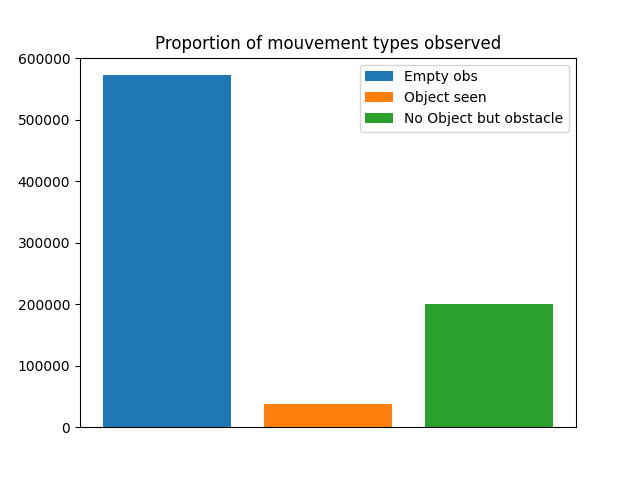
\includegraphics[scale = 0.5]{Proportions}
\end{center}	

	Pour palier à cela, on a donc renforcé l'apprentissage en pondérant la rétropropagation lors de l'apprentissage en fonction de la distance à l'objectif.

\begin{center}
	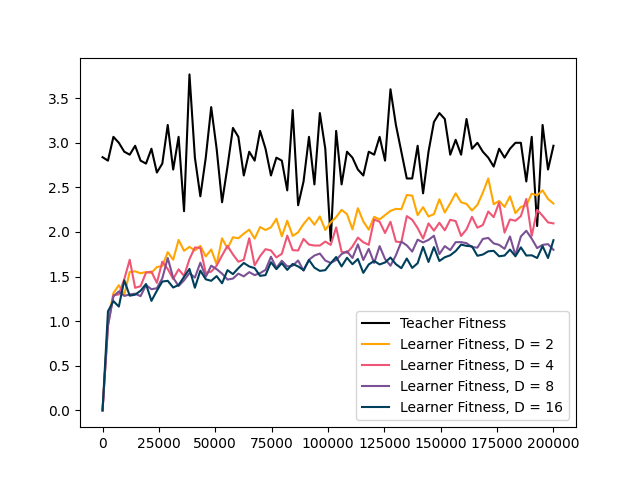
\includegraphics{averageComparisons}
\end{center}	
	
Cette méthode est, comme attendu, plus lente que la version ad-hoc. En revanche elle semble suivre une croissance continue. Il serait envisageable de poursuivre l'experience jusqu'à la stabilisation de la population.
	
\begin{center}
	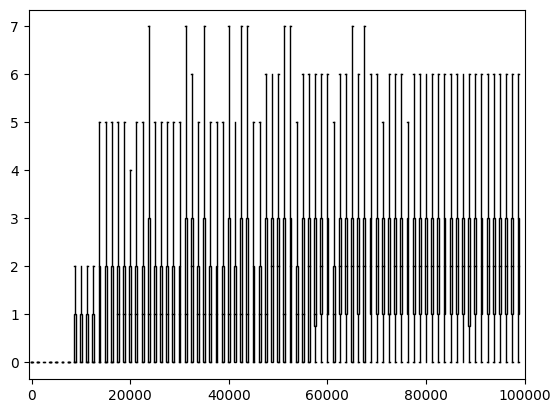
\includegraphics{learner_boxplot}
\end{center}	

	En permettant en plus l'apprentissage d'avoir lieu entre apprenants, on observe que la moyenne ne semble pas s'améliorer plus vite que dans l'expérience précédente. Néanmoins, l'ensemble de la population évolue de manière plus homogène.

    \section{Bibliographie}
//TODO
Nous recommandons l'usage de \href{https://fr.wikipedia.org/wiki/BibTeX}{BibTeX} pour la gestion de la bibliographie. Ajoutez les entrées correspondant à vos références dans le fichier \verb+resources/bib/references.bib+. Vous pouvez obtenir les entrées BibTeX sur \href{https://scholar.google.com}{Google Scholar} ou \href{https://dblp.uni-trier.de}{DBLP}. La commande \verb+\cite+ vous permet de citer une (ou plusieurs) référence(s) dans le document, par exemple \cite{pakin2020comprehensive,RusselNorvig}.

\chapter{Conclusion}

A première vue, l'apprentissage par comportement au sein d'un essaim de robots semble être une méthode prometteuse pour l'apprentissage à moindre coût.

Néanmoins, avant de pouvoir vraiment la comparer à d'autres méthodes existantes et la tester dans le monde réel, il faudrait déjà la tester avec la perte de connaissances qu'induit un changement de perspective.
\begin{center}
	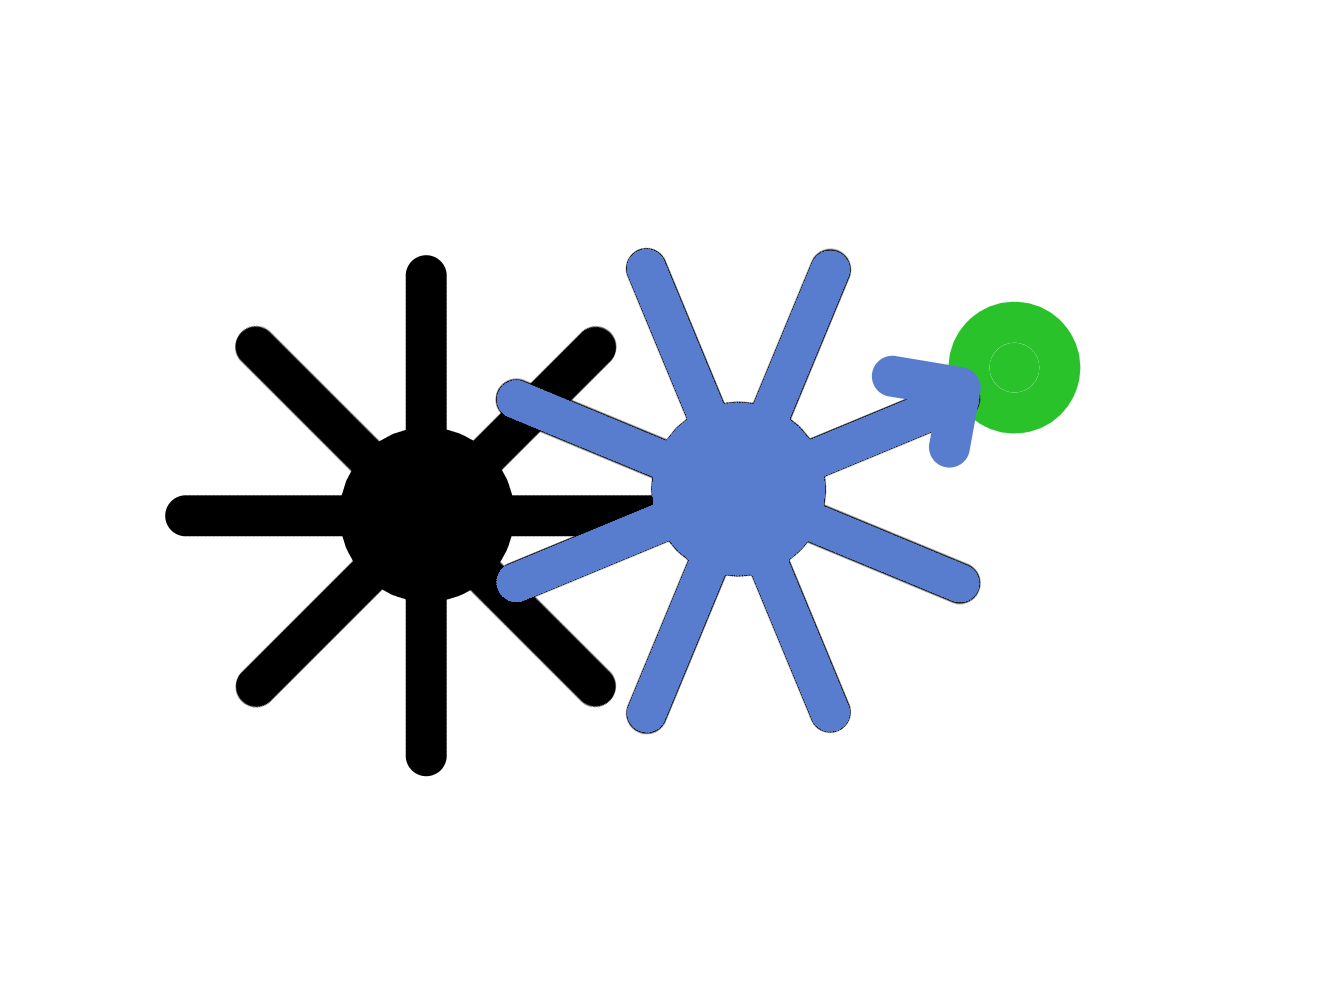
\includegraphics[scale = 0.5]{scheme.png}
\end{center}
\textit{Dans l'exemple ci-dessus, l'apprenant(en noir), ne voit pas l'objet(en vert) vers lequel se dirige l'expert(en bleu), pour lui l'expert ne détecte aucun objet à part l'apprenant.}

De plus, certaines de nos experiences n'ont pu avoir de résultats représentatifs par manque de temps. Ainsi, pour la poursuite de notre projet, nous devrions optimiser les différents codes pour permettre des expériences plus représentatives, pour ensuite pouvoir comparer nos résultats avec les algorithmes "state of the art"

    %\printbibliography

    \appendix

    \chapter{Cahier des charges}
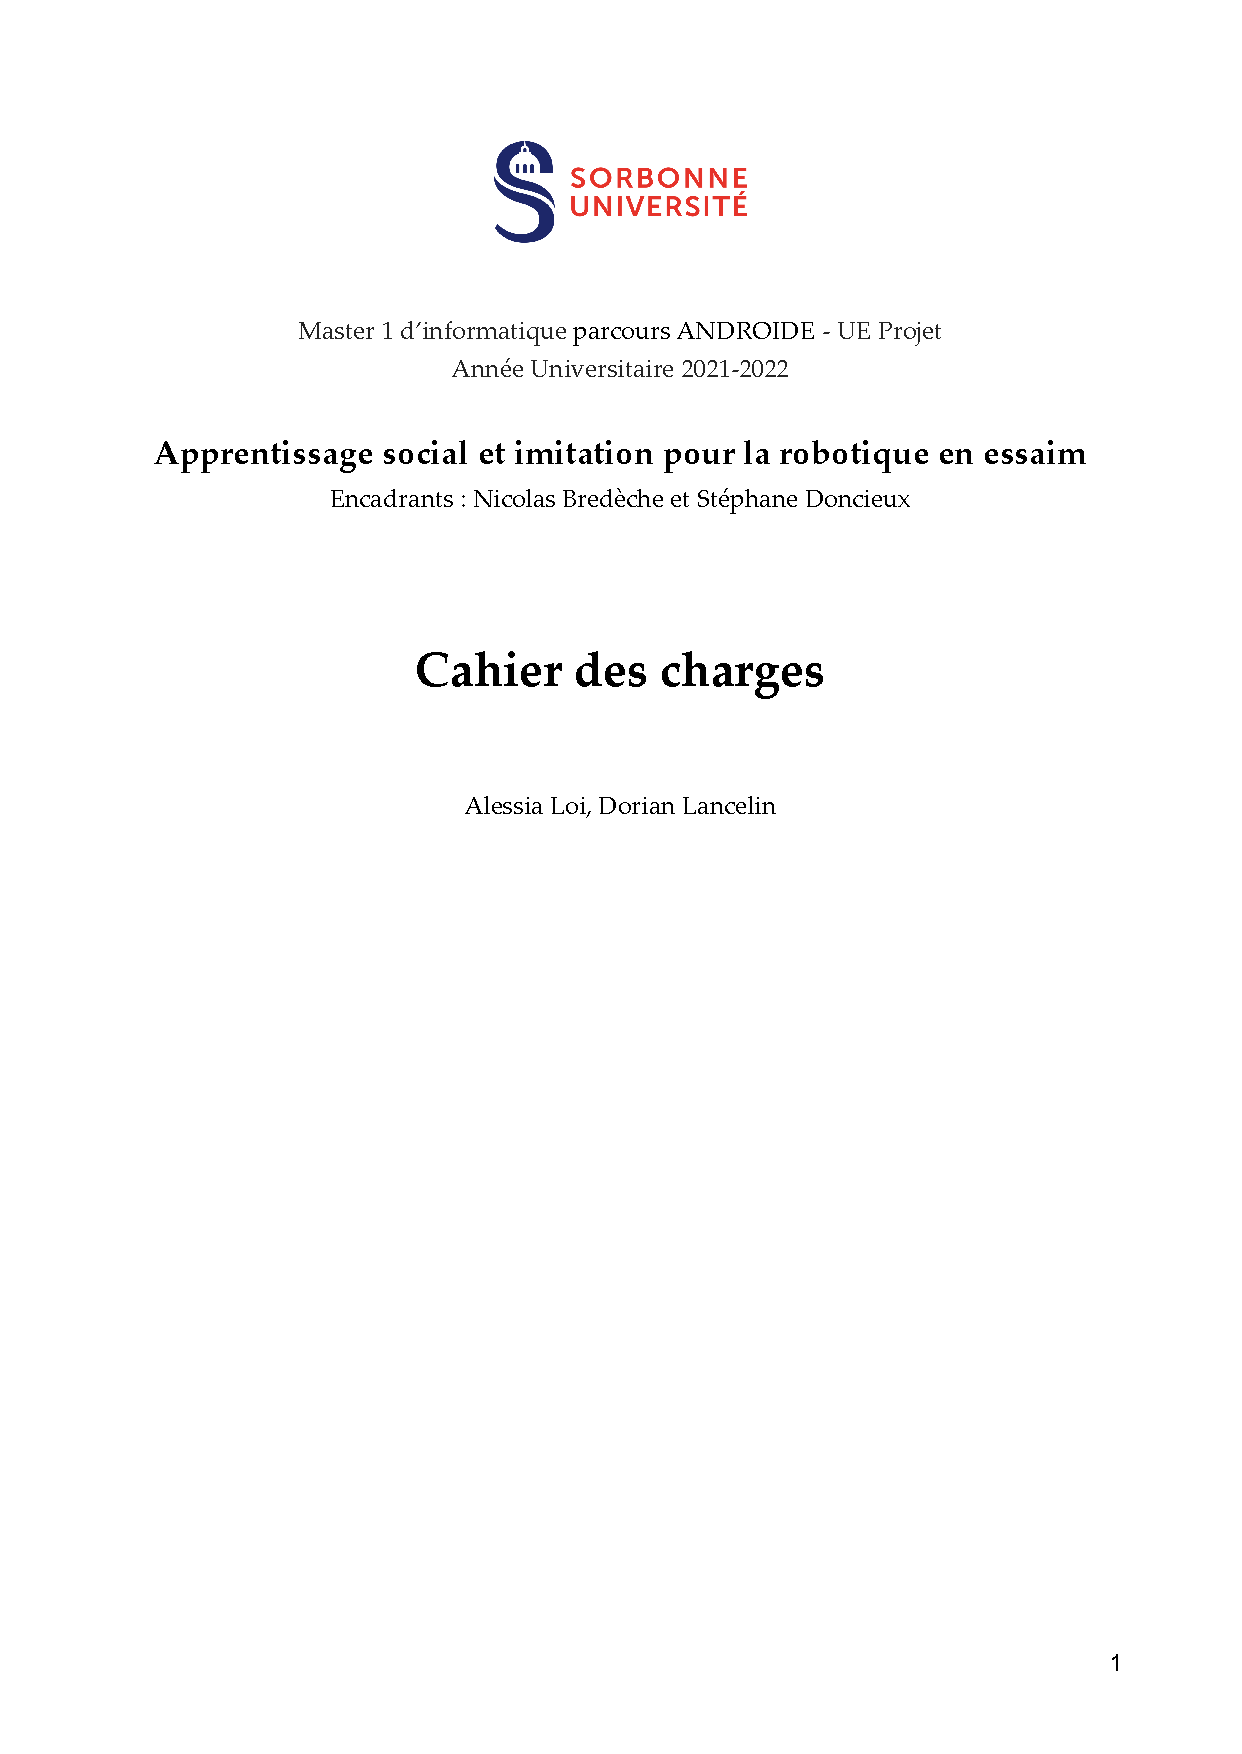
\includepdf[scale = 0.8,nup=2x2, pages=1-4]{CDC.pdf}
    \chapter{Manuel utilisateur}
     
     
    \subsection{Méthode par transmission de comportements}
    
    \begin{itemize}
        \item Se positionner sur le répertoire \textit{ASIRE\_project}
        
        \item Dans le fichier \textit{part2\_main\_diffusion.py}, en début de page, fixer les paramètres à utiliser :
        
        \begin{itemize}
        \item section \textbf{\textit{configuration file parameters}}. Fixer le nombre de individus experts \textit{nbExpertsRobots}, le nombre d'individus focaux \textit{nbNotExpertsRobots} et le nombre d'objets \textit{nbFoodObjects} pour l'expérience. Remarque : il ne faut pas modifier le fichier de configuration qui se trouve dans le répertoie \textit{config}.
        \item section \textbf{\textit{learning mode configuration}}. Choisir la mèthode d'apprentissage pour l'expérience courante : commenter la ligne de la mèthode à ne pas utiliser.
      \item section \textbf{\textit{parameters}}. Fixer le nombre total de steps \textit{nbSteps} de l'expérience et la taille de la base de données des individus \textit{maxSizeDictMyBehaviors}. Affecter \textit{True} à la variable \textit{learningOnlyFromExperts} pour limiter la possibilité de diffuser ses traces comportamentales aux seuls individus experts; affecter \textit{False} pour permettre à tous les individu de diffuser ses propres traces comportamentales.
            \item section \textbf{\textit{debug and plot parameters}}. Il est possible de visualiser les détails d'execution des algorithmes en affectant la valeur \textit{True} aux différentes variables \textit{debug\_*}.
            
        \end{itemize}
        
        Remarque : le fichier \textit{part2\_bestParameters.txt} conserve une copie des meilleurs paramètres testés lors des expériences.
        
        \item Exécuter le fichier \textit{part2\_main\_diffusion.py}.
    
    \end{itemize}

\end{document}
